\documentclass[12pt]{article}

% Layout.
\usepackage[top=1in, bottom=0.75in, left=1in, right=1in, headheight=1in, headsep=6pt]{geometry}

% Fonts.
\usepackage{mathptmx}
\usepackage[scaled=0.86]{helvet}
\renewcommand{\emph}[1]{\textsf{\textbf{#1}}}

% TiKZ.
\usepackage{tikz, pgfplots}
\usetikzlibrary{calc}
\pgfplotsset{compat = newest}
 
\pgfplotsset{my style/.append style={axis x line=middle, axis y line=
middle, xlabel={$x$}, ylabel={$y$}, axis equal }}

% Misc packages.
\usepackage{amsmath,amssymb,latexsym}
\usepackage{graphicx}
\usepackage{array}
\usepackage{xcolor}
\usepackage{multicol}
\newcolumntype{L}[1]{>{\raggedright\let\newline\\\arraybackslash\hspace{0pt}}m{#1}}
\newcolumntype{C}[1]{>{\centering\let\newline\\\arraybackslash\hspace{0pt}}m{#1}}
\newcolumntype{R}[1]{>{\raggedleft\let\newline\\\arraybackslash\hspace{0pt}}m{#1}}

% Commands to set various header/footer components.
\makeatletter
\def\doctitle#1{\gdef\@doctitle{#1}}
\doctitle{Use {\tt\textbackslash doctitle\{MY LABEL\}}.}
\def\docdate#1{\gdef\@docdate{#1}}
\docdate{Use {\tt\textbackslash docdate\{MY DATE\}}.}
\def\doccourse#1{\gdef\@doccourse{#1}}
\let\@doccourse\@empty
\def\docscoring#1{\gdef\@docscoring{#1}}
\let\@docscoring\@empty
\def\docversion#1{\gdef\@docversion{#1}}
\let\@docversion\@empty
\makeatother

% Headers and footers layout.
\makeatletter
\usepackage{fancyhdr}
\pagestyle{fancy}
\fancyhf{} % Clears all headers/footers.
\lhead{\baselineskip 30pt
%\emph{\@doctitle\hfill\@docdate}
\emph{\@docdate\hfill\@doctitle}
\ifnum \value{page} > 1\relax\else\\
\emph{Name: \rule{3.5in}{1pt}\hfill \@docscoring}\fi}
\rfoot{\emph{\@docversion}}
\lfoot{\emph{\@doccourse}}
\cfoot{\emph{\thepage}}
\renewcommand{\headrulewidth}{0pt}%
\makeatother

% Paragraph spacing
\parindent 0pt
\parskip 6pt plus 1pt

% A problem is a section-like command. Use \problem{5} to
% start a problem worth 5 points.
\newcounter{probcount}
\newcounter{subprobcount}
\setcounter{probcount}{0}
\newcommand{\problem}[1]{%
\par
\addvspace{4pt}%
\setcounter{subprobcount}{0}%
\stepcounter{probcount}%
\makebox[0pt][r]{\emph{\arabic{probcount}.}\hskip1ex}\emph{[#1 points]}\hskip1ex}
\newcommand{\thesubproblem}{\emph{\alph{subprobcount}.}}

% Subproblems are an enumerate-like environment with a consistent
% numbering scheme. 
% Use \begin{subproblems}\item...\item...\end{subproblems}
\newenvironment{subproblems}{%
\begin{enumerate}%
\setcounter{enumi}{\value{subprobcount}}%
\renewcommand{\theenumi}{\emph{\alph{enumi}}}}%
{\setcounter{subprobcount}{\value{enumi}}\end{enumerate}}

% Blanks for answers in normal and math mode.
\newcommand{\blank}[1]{\rule{#1}{0.75pt}}
\newcommand{\mblank}[1]{\underline{\hspace{#1}}}
\def\emptybox(#1,#2){\framebox{\parbox[c][#2]{#1}{\rule{0pt}{0pt}}}}

% Misc.
\renewcommand{\d}{\displaystyle}
% \newcommand{\ds}{\displaystyle}
\def\bc{\begin{center}}
\def\ec{\end{center}}
\def\be{\begin{enumerate}}
\def\ee{\end{enumerate}}


\doctitle{Math 251: Quiz 3}
\docdate{Jan 30, 2025}
\doccourse{UAF Calculus I}
\docversion{v-1}
\docscoring{\blank{0.8in} / 25}
\begin{document}
%\textbf{Please circle your instructor's name:} \hfill Leah Berman  \hfill   Jill Faudree\\

There are 25 points possible on this quiz. No aids (book, calculator, etc.)
are permitted.  {\bf Show all work for full credit.}

\problem{12} Consider the graph of the function $f$ below.
\begin{center}
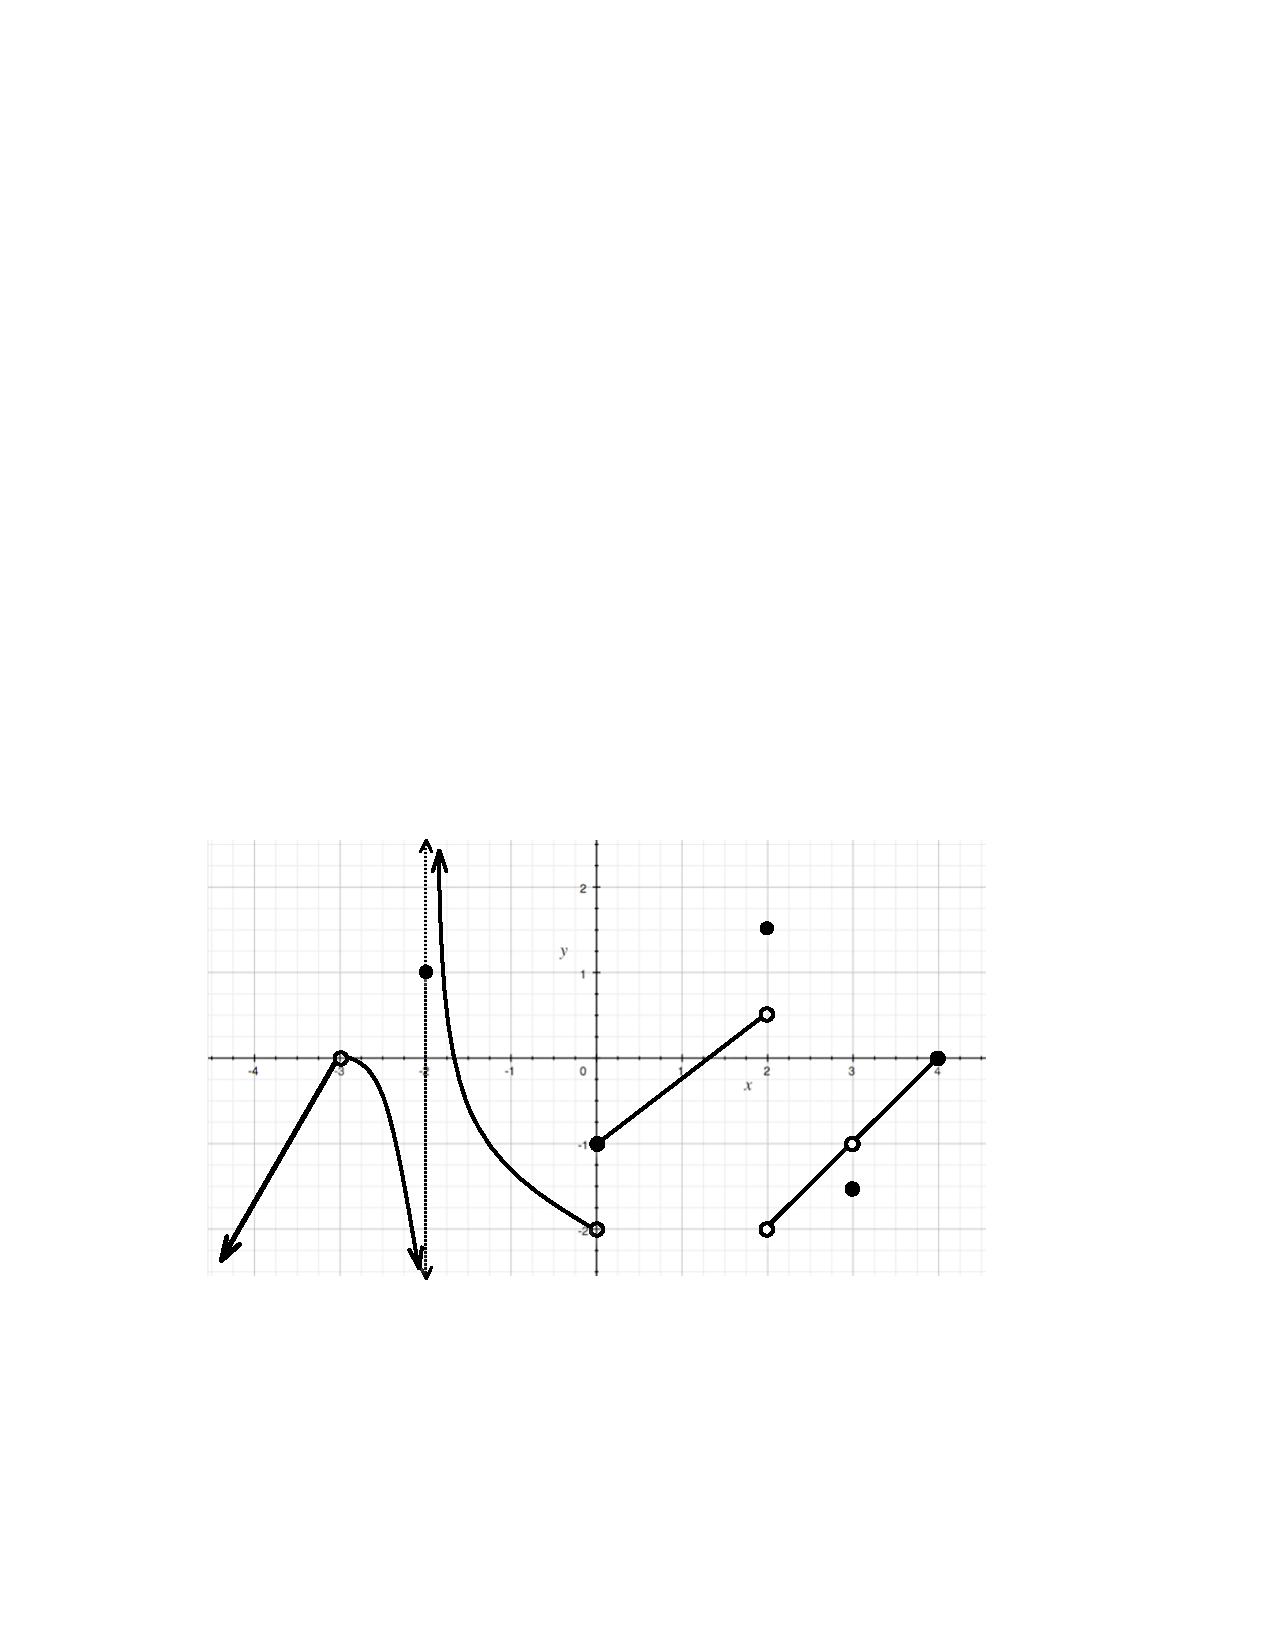
\includegraphics[width=5in]{LimitsGraph} 
\end{center}
Use the graph of $f$ to answer each question below. If the limit is infinite, indicate that with $\infty$ or -$\infty$. If the value does not exist or is undefined, write DNE.

\begin{center}
\begin{tabular}{L{2in}L{2in}L{2in}}
(a) $\displaystyle{\lim_{x\rightarrow -3}f(x)=}$&
(b) $\displaystyle{\lim_{x\rightarrow -2}f(x)=}$&
(c) $\displaystyle{\lim_{x\rightarrow 1}f(x)=}$ \\ [3em]
(d) $\displaystyle{\lim_{x\rightarrow -2^{+}}f(x)=}$&
(e) $\displaystyle{\lim_{x\rightarrow 2^{-}}f(x)=}$&
(f) $\displaystyle{\lim_{x\rightarrow 3^{-}}f(x)=}$\\[3em]
(g) $f(-3)=$&
(h) $f(2)=$&
(i) $f(3)=$
\end{tabular}
\end{center}

(j) Indicate \textbf{all} $x$-values for which the function $f$ is \textbf{not continuous}.\\

\underline{\hspace{15cm}}

%Use the graph to determine whether $f$ is continuous or not at the following values for $x$. State ``yes'' if it is continuous and ``no'' if it is not continuous.

%\begin{center}
%\begin{tabular}{L{2in}L{2in}L{2in}}
%(j) $x=0$ \underline{\hspace{2cm}} &
%(k) $x=1$ \underline{\hspace{2cm}} &
%(l) $x=3$ \underline{\hspace{2cm}} \\ [3em]
%\end{tabular}
%\end{center}

\newpage


\problem{9} Evaluate the following limits. Justify your answers.
\begin{subproblems}
\item $\d \lim_{x \rightarrow 2} \, x^2-3x+5$
  \vfill

\item $\d \lim_{x \rightarrow 4} \, \frac{x^2-2x-8}{x^2-5x+4}$
  \vfill

\item $\d \lim_{\theta \rightarrow \pi} \, \frac{\tan\theta}{\sin\theta}$ \hspace{5cm} $\d \left(\text{Hint: } \tan\theta = \frac{\sin\theta}{\cos\theta}\right)$
  \vfill

%\item $\d \lim_{x \rightarrow 0} \, \frac{x+3}{x^2+6x+9}$
%  \vfill

\end{subproblems}
\newpage

\problem{4} Determine whether or not the given function is
continuous at $x=5$. \textbf{Justify your answer using limits.}\\

   \begin{equation*}
    f(x) =
    \begin{cases}
      \frac{x+3}{x-1} & \text{ if } x <5 \\
      x^2-3x-8 & \text{ if } x \geq 5
    \end{cases} %\text{ , at } x=5
  \end{equation*}
  \vfill


%\begin{subproblems}
%\item \begin{equation}
%    f(x) =
%    \begin{cases}
%      x^2-4 & \text{ if } x > 3 \\
%      2x+1 & \text{ if } x \leq 3
%    \end{cases} \text{ , at } x=3
%  \end{equation}
%  \vfill
  
%\item \begin{equation}
%    f(x) =
%    \begin{cases}
%      \frac{x+3}{x-1} & \text{ if } x <5 \\
%      x^2-3x-8 & \text{ if } x \geq 5
%    \end{cases} \text{ , at } x=5
%  \end{equation}
%  \vfill

% \end{subproblems}

%\newpage
\problem{2} BONUS: Does the equation $2x^7 - x^5 = 3x^{31} + 5x^{13} + 2x^7 +
x^3$ have a solution on the interval $[-1,1]$? Justify your answer.
	
\vfill
	
\end{document}
%%% Local Variables:
%%% mode: LaTeX
%%% TeX-master: t
%%% End:
